\subsection{Earth and Moon Crossings}
\label{sec:earth_moon_crossings}
\begin{figure}[!tb]
	%	\includegraphics{}
	\centering
	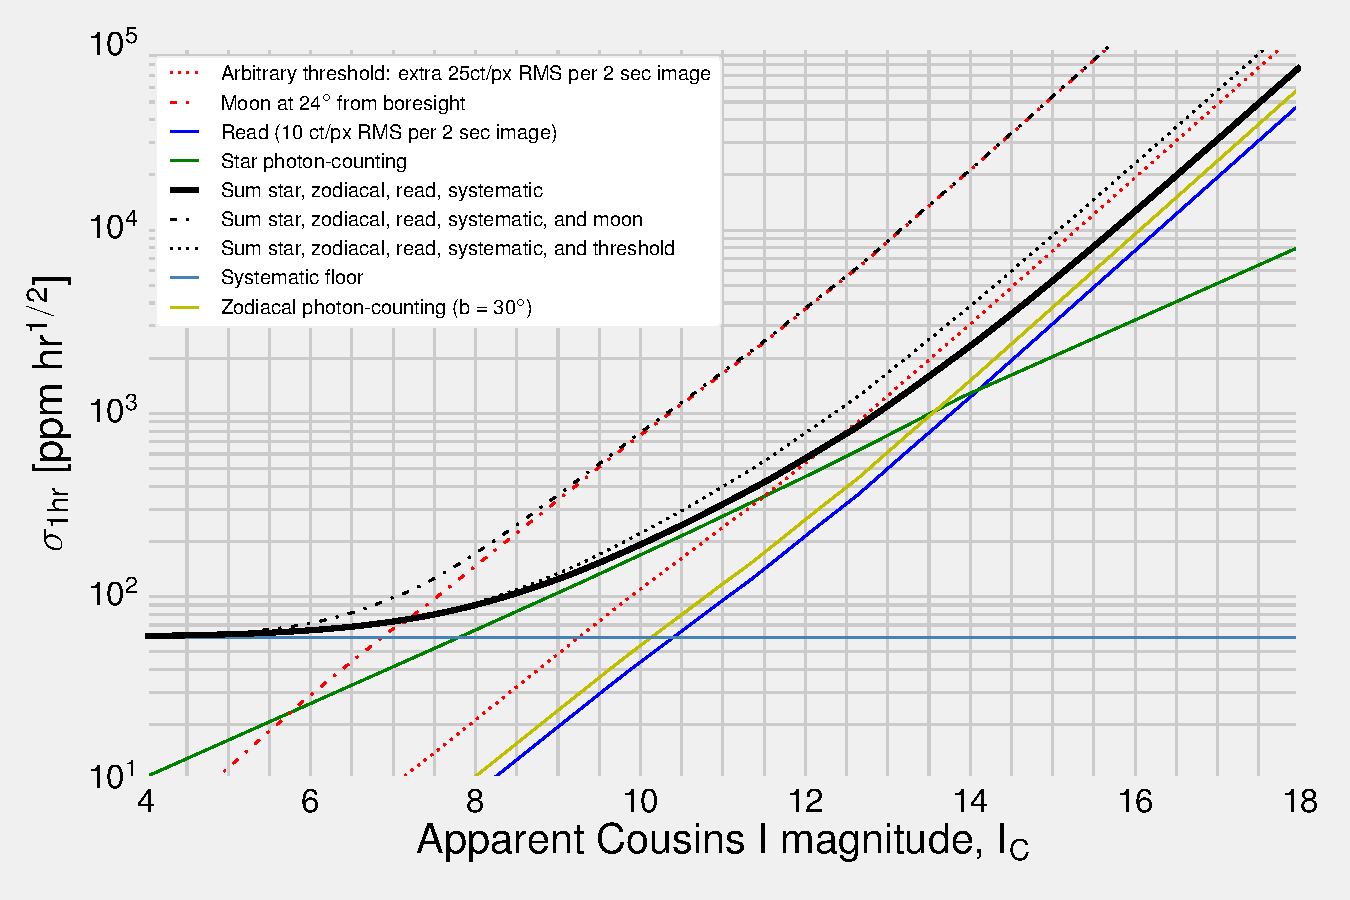
\includegraphics{figures/precision_memo.pdf}
	\caption{Relative precision in measured flux over a one hour integration 
	time (scatter from contaminating background stars and PRF centroid offsets 
	ignored). The noise sources described by~\protect\citet{Sullivan_2015} are 
	solid thin lines.
	The dashed-dot lines correspond to additional background flux from the Moon 
	when it is $24^\circ$ from a camera's boresight.	
	The dotted lines correspond to a threshold, $F_\mathrm{thresh}\equiv 
	300\,\mathrm{ct/px/s}$, that we use to flag Moon and Earth contamination in 
	\tesss field of view (see text).
	Zodiacal background is plotted for an ecliptic latitude of $30^\circ$ using 
	Eq. 21 of~\protect\citet{Sullivan_2015}}
	\label{fig:noise_with_moon}
\end{figure}

When the Earth or Moon passes through \tesss camera fields they can
flood the CCD pixels to their full well capacity ($\sim2\times10^5$
photoelectrons).  Precision differential photometry becomes impossible
in any pixels that are directly hit during these crossings.  Even when
the body (Earth or Moon) is not directly in the camera's field of
view, its light scatters off the interior of spacecraft's lens hood
and acts as a background source of contaminating flux across many of
the cameras\footnote{A detailed model for this process is not yet
  available.}.  
The Poisson noise in the number of photons
arriving from the Earth or the Moon in such a scenario degrades \tesss
photometric performance.   

We first illustrate with an example.
When the Moon is $24^\circ$ from a camera boresight the lens hood 
is expected to suppress $1/100^\mathrm{th}$ of a mean 
$3\times10^6\,\mathrm{ct/px}$ (per 2 second image) from incoming 
moonlight\footnote{Our model for suppression as a function of angle is 
appended in Fig.~\ref{fig:lens_hood_suppression}. We implicitly assume 100\% 
quantum efficiency, so photons, electrons, and counts are interchangeable; 
$1\,\mathrm{ph} = 1\,\mathrm{e^{-1}} = 1\,\mathrm{ct}$.}.
Thus a mean flux of $3\times10^4\,\mathrm{ct/px}$ reaches the cameras per 
image. 
Assuming the arrival of these photons is Poissonian, the additional RMS is 
then $173\,\mathrm{ct/px}$ per 2 second image.
Including this additional variance in the quadrature sum of variances of all 
noise sources, Fig.~\ref{fig:noise_with_moon} shows that this background 
is the dominant noise source for stars with $I_c \gtrsim 7$ -- nearly all 
target stars.
While the effect's magnitude is highly dependent on the angle between a 
camera's
boresight and the Moon or Earth, the general picture is that for field angles 
$\theta \lesssim25^{\circ}$, the impact can be severe.

Separately from our planet detection simulation, we study these 
crossings in a dynamical simulation based on JPL NAIF's standard SPICE toolkit.
Given a nominal launch date (we assume Dec 20, 2017), this code determines 
\tesss orbital phasing throughout its entire mission. 
At every time step of the three-body orbit, we calculate the distance between 
\tess and the other two bodies of interest, and the separation angles among 
each of the four cameras and each of the two bodies (eight angles in total). 
The spacecraft's inclination oscillates in the simulation as it will in 
reality.

Taking the Earth and Moon's integrated disk brightnesses as fixed 
values\footnote{The full moon's apparent magnitude is $I_\moon \approx -13.5$. 
Scaling from photon fluxes tabulated in~\citet{winn_photonflux_2013}, this 
gives $2.5\times10^{13}\ \mathrm{ct/s}$. Averaging over the number of pixels 
in the focal plane array, 
this gives a mean additional flux per image of $3\times10^6\ \mathrm{ct/px}$.
The Earth will contribute a mean flux $\sim {80}$ times greater.
This substantiates the claim that the Earth and Moon flood the cameras to 
their full well capacity. 
The effect on observing precision is appended in 
Fig.~\ref{fig:outage_vs_background}.} we use a model for scattered light 
suppression from 
the \tess lens hoods (Fig.~\ref{fig:lens_hood_suppression}) to compute the 
mean photon flux from each of these bodies onto each of the cameras throughout 
the orbit. We then compute the corresponding variance in incoming flux, and 
compare it to \tesss noise budget, similar to the example in 
Fig.~\ref{fig:noise_with_moon}.

To evaluate the cumulative impact of Earth and Moon crossings on \tesss 
Primary and Extended Missions we ask: for each camera, what fraction of the 
total observing time is \tess unable to operate at desired photometric 
precision because of Earth and Moon crossings?
An upper limit for what we mean by `unable to operate at desired photometric 
precision' is when terrestrial or lunar flux make it impossible to observe a sizable portion of the stars in the \tess target star catalog with reasonable precision.
Following our example of when the Moon is $24^\circ$ from the camera boresight, 
the appended Fig.~\ref{fig:outage_vs_background} shows that $\sim$50\% of the 
stars that could be observed at sub-mmag precision over an hour no longer can.
This of course depends on the target star catalog's apparent magnitude 
distribution (Fig.~\ref{fig:fig17_replica}), and the cutoff of `sub-mmag 
precision over an hour' is arbitrarily selected.

\begin{figure}[!t]
	\centering
	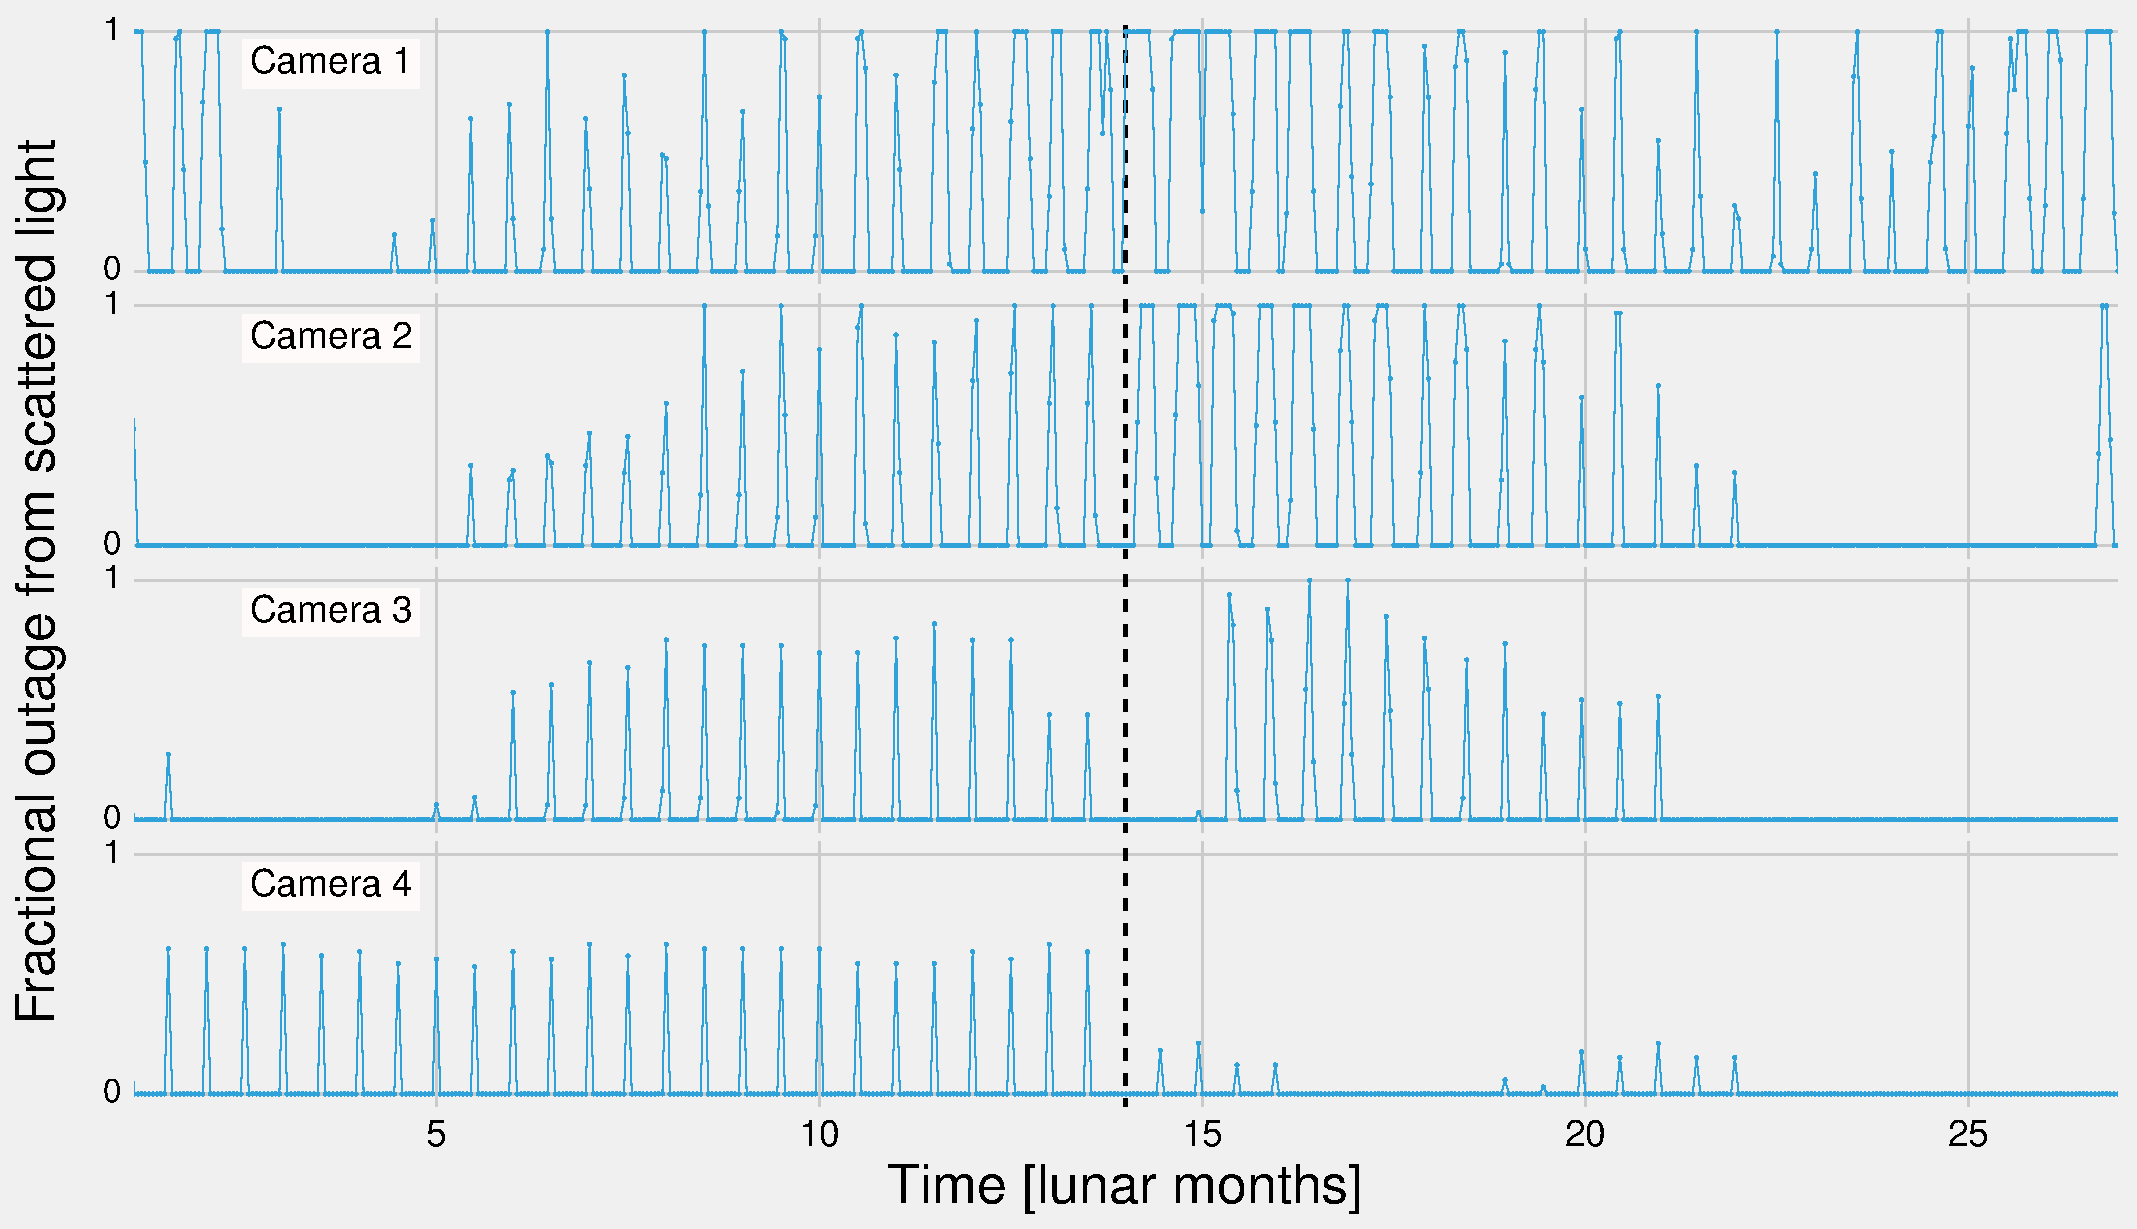
\includegraphics[angle=90,width=1.05\textwidth]{figures/outage_earth_moon_primary_panels.pdf}
	\caption{`Outage' caused by direct or scattered Earth- or Moonlight as a 
	function of time in \tesss orbit.
	Specifically, the $y$-axis shows the probability of having a polluted frame 
	with mean incident flux $>300\,\mathrm{ct/px/s}$ in a time-step bin of 
	1/20$^\mathrm{th}$ of an 
	orbit (where the probability is the number of polluted frames divided by 
	the total number of frames in that bin).
	The mean of this outage across any given year is used to compute the number of dropped fields in Table~\protect\ref{tab:dropped_fields}, which should then be an upper bound to the impact of Earth and Moon crossings.
	In this plot, the first year of observations are in the southern ecliptic 
	hemisphere. The dashed line marks the beginning of `Year 2' (northern 
	hemisphere). 
	\tess completes two orbits per lunar month.
	The worst fractional outage per orbit is in Camera 1, which 
	points towards the ecliptic, over the first $\sim\!5$ orbits of the second 
	year.
	The plot has `spikes' because outages only occur over a small 
	fraction of \tesss orbit when the relevant orbits align.}
	\label{fig:earth_moon_primary}
\end{figure}
%\clearpage
\begin{figure}[!t]
	\centering
	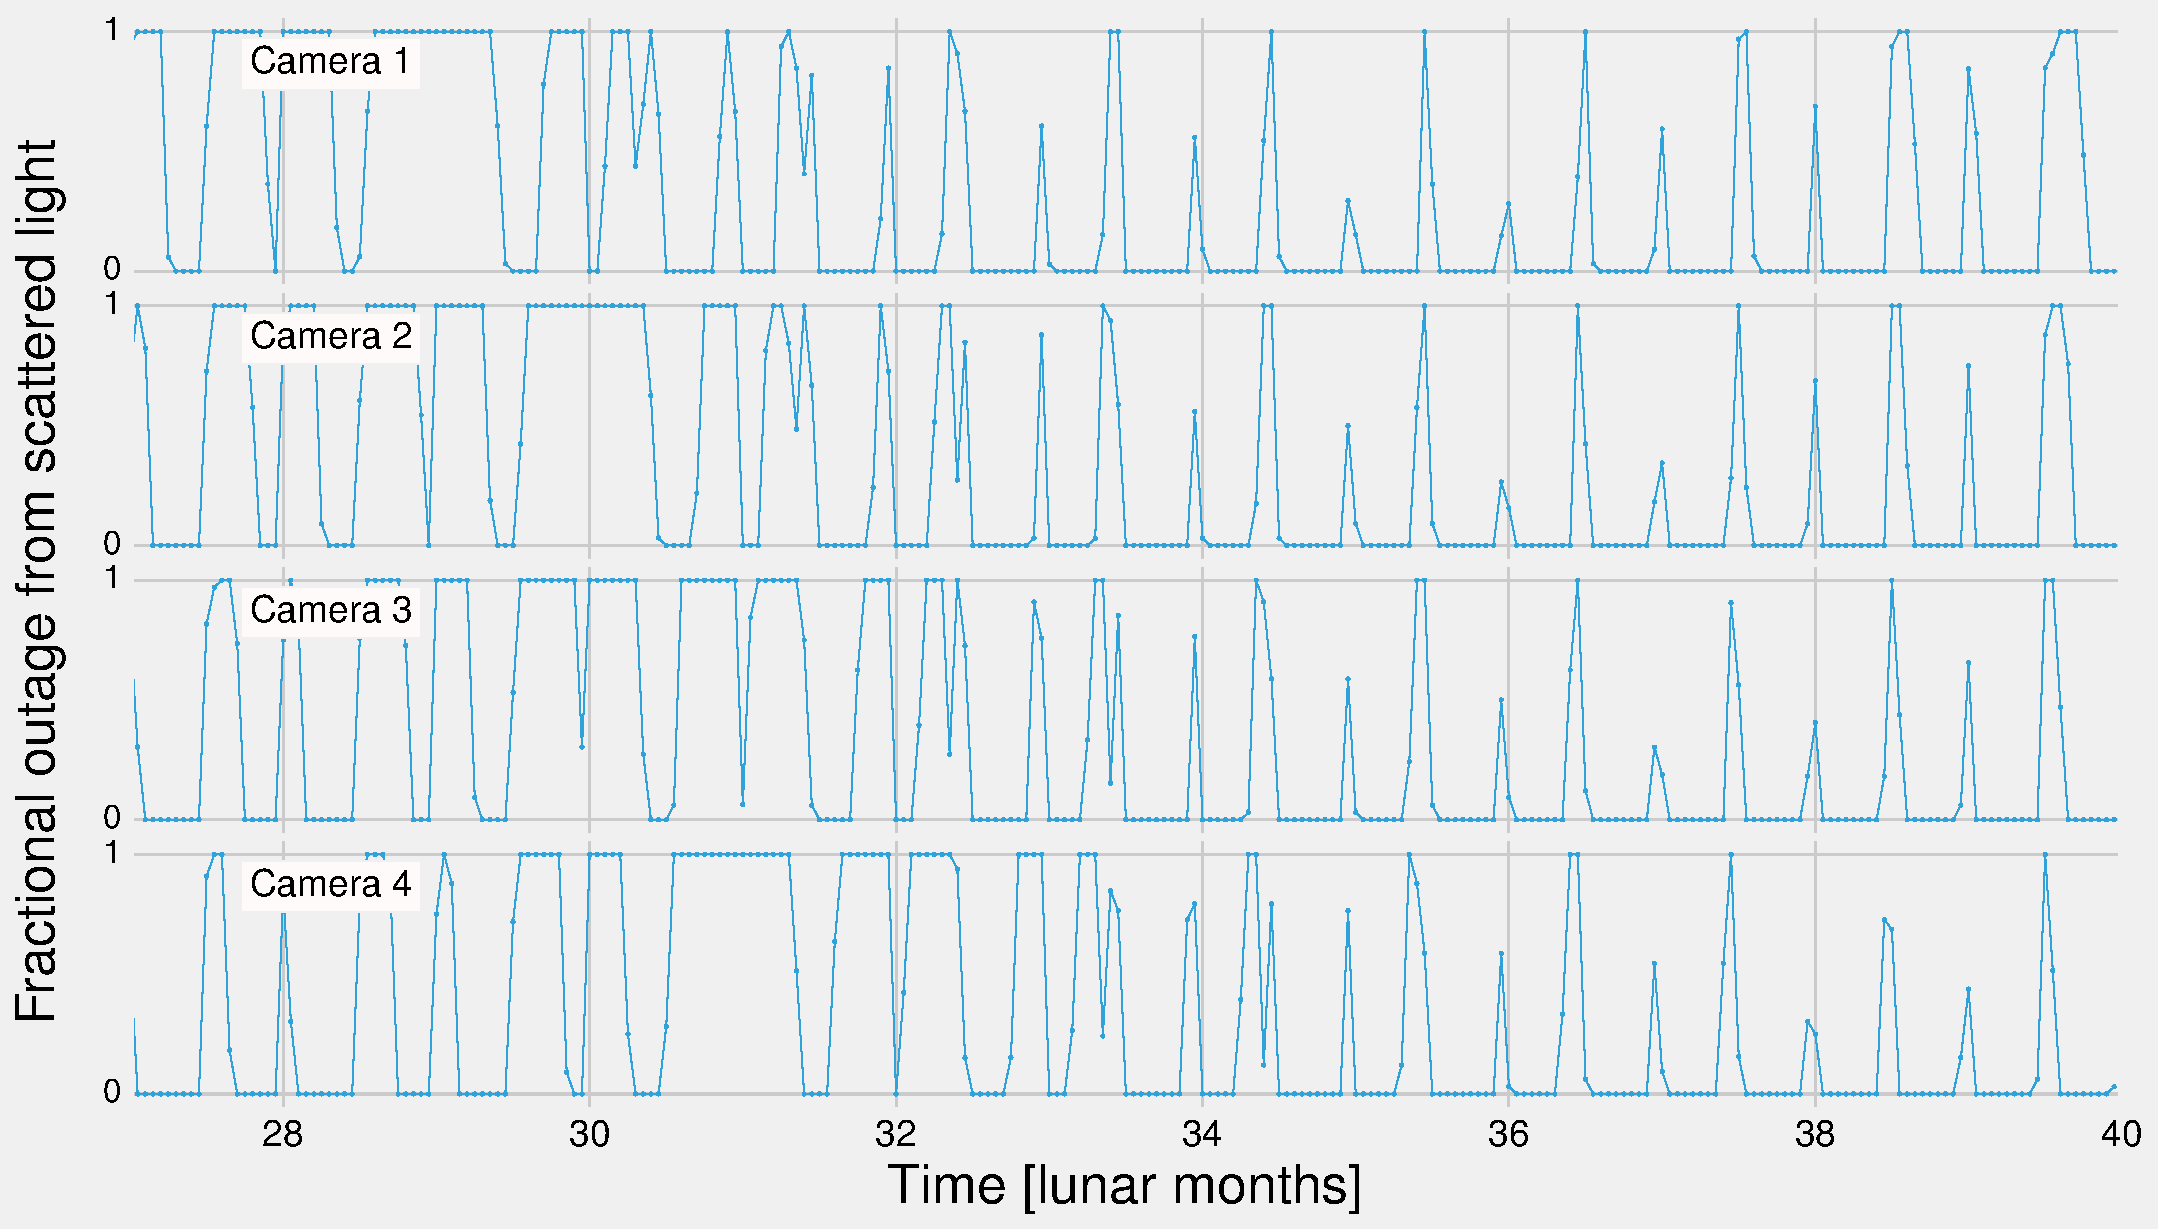
\includegraphics[angle=90,width=1.05\textwidth]{figures/outage_earth_moon_ecliptic_ext_panels.pdf}
	\caption{Same as Fig.~\protect\ref{fig:earth_moon_primary}, except showing 
	a hypothetical third year in which \tess observes the ecliptic with the 
	cameras' long axis along the ecliptic plane for the entire year. The latter 
	half of the year experiences far less Earth and Moon interference than the 
	first half. Considering it implausible that we would opt to sacrifice such 
	a large fraction of our observing time, we study the \elong\:and 
	\eshort\:scenarios instead, as their observations avoid this effect during 
	the first $\sim5$ months.}
	\label{fig:earth_moon_elong}
\end{figure}
\begin{table}[!tb]
	\centering
	\begin{tabular}{ | l | l | l | l | l | }
		\hline
		\ & Camera 1 & Camera 2 & Camera 3 & Camera 4 \\ \hline
		\multicolumn{1}{|c|}{Year 3 selected} & \  & \  & \  & \  \\ \hline
		\npole & 0 & 0 & 0 & 0 \\ \hline
		\nhemi & 2 & 1 & 0 & 0 \\ \hline
		\shemiAvoid & 2 & 0 & 0 & 0 \\ \hline
		\elong & 1 & 1 & 1 & 1 \\ \hline
		\eshort & 0 & 1 & 1 & 0 \\ \hline
		\hemis & 1 & 1 & 0 & 0 \\ \hline
		\multicolumn{1}{|c|}{Year 3 omitted} & \  & \  & \  & \  \\ \hline
		\texttt{pole\,(south)}  & 0 & 0 & 0 & 0 \\ \hline
		\texttt{hemi\,(south)} & 1 & 0 & 0 & 0 \\ \hline
		\texttt{hemi+ecl\,(south)} & 4 & 3 & 0 & 0 \\ \hline
		\texttt{ecl\_long\,(1yr)} & 4 & 4 & 4 & 4 \\ \hline
		\texttt{ecl\_short\,(1yr)} & 1 & 3 & 4 & 2 \\ \hline
		\texttt{allsky\,(poles)} & 0 & 0 & 0 & 0 \\ \hline
		\multicolumn{1}{|c|}{Primary Mission} & \  & \  & \  & \  \\ \hline
		\texttt{hemi\,(south year 1)} & 2 & 1 & 0 & 0 \\ \hline
		\texttt{hemi\,(north year 2)} & 4 & 2 & 0 & 0 \\ \hline
	\end{tabular}
	\caption{Number of sectors (of 13 per year) `dropped' due to the Earth and 
	Moon crossings in both selected and omitted Extended Missions, with those 
	of the Primary Mission for reference. The method of `dropping' fields 
	(which neglects the temporal nature of the crossings, discussed in the 
	text) gives an approximate sense of the cumulative impact of Earth and Moon 
	crossings. 
		Scenarios with \texttt{(south)} appended refer to their counterparts in the southern ecliptic hemisphere.
		\texttt{ecl\_long\,(1yr)} corresponds to a full year with the long axis 
		of \tesss field of view along the ecliptic, while 
		\texttt{ecl\_short\,(1yr)} corresponds to the same, but with the short 
		axis along (long axis perpendicular to) the ecliptic. These scenarios 
		are neglected because their outages are time-correlated (see 
		Fig.~\protect\ref{fig:earth_moon_elong}).
		\texttt{allsky\,(poles)} would be a scenario that observes in the manner of \hemis, but only on the ecliptic poles as in \npole.}
	\label{tab:dropped_fields}
\end{table}


Developing a detailed model of how these crossings impact \tesss photometry is beyond the scope of this work.
To account at least qualitatively for their effect in our simulation we adopt a 
simple approximation: we impose that a camera has an `outage' if there are over 
$F_\text{thresh}\equiv300\ \text{ct/px/s}$.
This is roughly twice the maximal zodiacal background noise, which in our model 
ranges from $48$-$135\,\mathrm{ct/px/s}$ (see \citetalias{Sullivan_2015} Sec 
6.4.1). At an ecliptic latitude of $30^\circ$, Eq. 21 of 
\citetalias{Sullivan_2015} gives $75\,\mathrm{ct/px/s}$, or about 
$F_\mathrm{thresh}/4$.

We then compute the time-averaged fraction of each observing sector for which \tesss cameras remain above this threshold. 
A given sector has $\sim660$ hours of observing time over two spacecraft orbits.
As an example, suppose that $220$ of these hours had the Earth, the Moon, or both shining with a background flux $F > F_\text{thresh}$. 
This would correspond to a fractional outage of $1/3$. 
We then compute the mean of this fractional outage across all 13 annual sectors to derive a `mean camera outage' for each proposed pointing scenario.
We then approximate the effect of Earth and Moon crossings by selectively 
omitting the closest integer number of observing sectors corresponding to the 
`mean camera outage' described above.
For instance, if the `mean camera outage' was 17\% of \tesss observing time over a given year, we would omit the 2 (of 13) observing sectors that suffer the greatest number of lost hours, for that given camera.
The relevant number of omitted sectors is shown in Table~\ref{tab:dropped_fields}; an example of the resulting spatial distribution of detected planets is shown in Fig.~\ref{fig:skymap_nhemi}.


As mentioned in Sec.~\ref{sec:planet_detection_model}, our planet detection 
simulation is not explicitly time-resolved; it takes the ecliptic coordinates 
of camera fields for each orbit as input to compute the observed baselines for 
each star in our galactic model.
While our procedure ignores the temporal nature of the `outages' (which is 
shown resolved over time-steps of 1/20$^\mathrm{th}$ of an orbit in 
Figs.~\ref{fig:earth_moon_primary} and~\ref{fig:earth_moon_elong}), it gives a 
sense of the cumulative impact of Earth and Moon crossings over 
the course of a year, which is sufficient for the purposes of this study.

%Our approximation is `conservative' in the sense that 
The additional background corresponding to $F_\mathrm{thresh}=300\ 
\mathrm{ct/px/s}$ becomes a noticeable noise source ($\gtrsim 1.5\times$ lower
precision) for targets with $I_c \gtrsim 12$ (cf.
Fig.~\ref{fig:noise_with_moon}).
This is roughly half of the target stars, with the greatest impact on the M 
dwarf sub-sample.
By approximating all of the relevant time as an `outage' lost across all stars 
(even for the bright ones for which the additional scatter is subsumed by 
other noise sources), our simulation results might be more sensitive to 
scattered light than \tess will be in reality.
However, scattered light might have a non-Poisson component, and is   expected 
to 
be non-uniformly distributed across each focal plane as the Moon or Earth 
moves relative to \tesss pointing.
%would make removing scattered light in post-processing more difficult, and 
This could make the effect worse than simulated.

The impact of this approximation on the planet yields of the Primary and 
Extended Missions are discussed in 
Secs.~\ref{sec:results_from_primary_missions} and~\ref{sec:results_from_all_extended_missions}
 respectively.
The summarized result is that this model of Earth and Moon crossings leads to 
$\lesssim 10\%$ fewer $R_p<4R_\oplus$ planet detections in the Primary Mission 
compared to the case of 
not accounting for the crossings at all.
%There is thus little reason to raise our low threshold, given that the 
%magnitude of the effect is so small.
%Moreover, the Earth and Moon crossings typically last for a small fraction of 
%an orbit (Fig.~\ref{fig:earth_moon_primary}). If the timescales required for 
%the cameras to `re-settle' after the crossings are small compared to orbital 
%timescales, our approach may over-estimate the effect's importance even 
%further.
Detailed models of this process remain to be developed during the spacecraft's 
commissioning period.

% I think this might be a bit better than it sounds because of how the earth/moon crossings are phased in the orbits. They're only happening for at worst ~1/2 of an orbit (see https://drive.google.com/folderview?id=0B2941jxrlPq0Z0tQZnRpd3pVOHc&usp=drive_web), but at roughly the same half across adjacent sectors. I.e. it's the same patches of sky, roughly, that aren't being observed across adjacent sectors, so just dropping the entire sector isn't as bad as you might think on first guess. It's admittedly somewhat sketch.

%A detailed model of this effect would take this dynamical simulation and incorporate it with the extant \tess instrument model to produce full simulated images of the \tess fields every 2 minutes over the course of a specified mission.
%Reduction to postage stamps and full frame images could be modeled in a `true' sense from these simulated images.
%The main apparatus of the planet detection simulation -- the process of creating planets, selecting transiting planets, and producing small images with the transiting planet signal injected, and computing a SNR for these  -- this is a somewhat long process. Maybe more like a masters thesis, and a phd thesis if you did it right.









